\documentclass[ChapterTOCs,krantz2]{krantz} % Use krantz2 for 7" x 10" trim size

\usepackage[utf8]{inputenc}
\usepackage{graphicx}
\usepackage{subfigure}
\usepackage{epigraph}
%-----------------------------------------------------------------------------
% Special-purpose color definitions (dark enough to print OK in black and white)
\usepackage{color}
\usepackage{amsthm}

% A few colors to replace the defaults for certain link types
\definecolor{orange}{cmyk}{0,0.4,0.8,0.2}
\definecolor{darkorange}{rgb}{.71,0.21,0.01}
\definecolor{darkgreen}{rgb}{.12,.54,.11}

%-----------------------------------------------------------------------------
% The hyperref package gives us a pdf with properly built
% internal navigation ('pdf bookmarks' for the table of contents,
% internal cross-reference links, web links for URLs, etc.)
%\usepackage{hyperref}

\usepackage{url}

%% Define a new 'leo' style for the package that will use a smaller font.
\makeatletter
\def\url@leostyle{%
  \@ifundefined{selectfont}{\def\UrlFont{\sf}}{\def\UrlFont{\small\ttfamily}}}
\makeatother
%% Now actually use the newly defined style.
\urlstyle{leo}

\newcommand{\blockpar}[1]{\vspace*{3mm} \noindent \textbf{#1}}

%-----------------------------------------------------------------------------
%
% Commands for annotating the docs with fixme and inter-author notes.  See
% below for how to disable these.
%
% Define a \fixme command to mark visually things needing fixing in the draft,
% as well as similar commands for each author to leave initialed special
% comments in the document.
% For final printing or to simply disable these bright warnings, copy
% (there's a target macros_off' in the makefile that does this) the file
% macros_off.tex to macros.tex
\usepackage{amssymb}

\newcommand{\fix}[1] { \textcolor{red} {
{\fbox{ {\bf Fix:} \ensuremath{\blacktriangleright }} {\bf #1}
\fbox{\ensuremath{\blacktriangleleft} } } } }

% And similarly, one (less jarring, with fewer symbols and no boldface) command
% for each one of us to leave comments in the main text.
\newcommand{\fperez}[1] { \textcolor{blue} {
\ensuremath{\blacklozenge} {\bf fperez:}  {#1}
\ensuremath{\blacklozenge} } }

\newcommand{\jarrod}[1] { \textcolor{darkgreen} {
\ensuremath{\bigstar} {\bf jarrod:}  {#1}
\ensuremath{\bigstar} } }

\newcommand{\mref}[1] { \textcolor{darkorange} {
\ensuremath{\blacksquare} {\bf missing ref:}  {#1}
\ensuremath{\blacksquare} } }

%% Uncomment these to turn all the special marker commands off
%\renewcommand{\fix}[1]{}
%\renewcommand{\fperez}[1]{}
%\renewcommand{\jarrod}[1]{}
%\renewcommand{\mref}[1]{}

\begin{document}

\title{Implementing Reproducible Research}
\author{Dummy author}
\chapter*{Dummy chapter needed for the \textbackslash chapterauthor command to work later}

\mainmatter

\chapterauthor{K. Jarrod Millman}{Division of Biostatistics\\
School of Public Health\\
University of California, Berkeley}
\chapterauthor{Fernando Pérez}{Henry H. Wheeler Jr. Brain Imaging Center\\
Helen Wills Neuroscience Institute\\
University of California, Berkeley\\
\\
\begin{flushright}
Dedicated to the memory of John~D.~Hunter~III, 1968-2012.
\end{flushright}}

\chapter{Developing open source scientific practice}


\section{Introduction}\label{intro}

Computational tools are at the core of modern research. In addition to
experiment and theory, the notions of simulation and data-intensive discovery
have emerged as third and fourth pillars of science \cite{4th-paradigm}.
Today, even theory and experiment are computational: experimental work requires
computing (whether in data collection, preprocessing, or analysis) and
theoretical work requires symbolic manipulation and numerical exploration to
develop and refine models. Scanning the pages of any recent scientific journal,
one is hard-pressed to find an article that does not depend on computing for
its findings.

Yet, for all its importance, computing receives perfunctory attention in the
training of new scientists and in the conduct of everyday research.  It is
treated as an inconsequential task that students and researchers learn ``on the
go'' with little consideration for ensuring computational results are
trustworthy, comprehensible, and ultimately a secure foundation for
reproducible outcomes.  Software and data are stored with poor organization,
little documentation, and few tests.  A haphazard patchwork of software tools
is used with limited attention paid to capturing the complex workflows that
emerge.  The evolution of code is not tracked over time, making it difficult to
understand what iteration of the code was used to obtain any specific result.
Finally, many of the software packages used by scientists in research are
proprietary and closed-source, preventing complete understanding and control of
the final scientific results.

We argue that these considerations must play a more central role in how
scientists are trained and conduct their research. Our approach grows out of
our experience as part of both the research and the open source scientific
Python communities.  We begin (§~\ref{sec:research}) by outlining our vision
for the scientific software development in everyday research. In the remaining
sections, we provide specific recommendations for computational work.  First,
we describe the routine practices (§~\ref{sec:practice}) that should be part of
the daily conduct of computational work. We next discuss tools and practices
developed by open source communities to enable and streamline collaboration
(§~\ref{sec:collaboration}). Finally, we present an approach to developing and
communicating computational work that we call literate computing in contrast to
the more mature approach of literate programming (§~\ref{sec:communication}).

\section{\label{sec:research}Computational research}

Consider a researcher using Matlab for prototyping a new analysis method,
developing high-performance code in C, post-processing by twiddling controls in
a Graphical User Interface (GUI), importing data back into Matlab for
generating plots, polishing the resulting plots by hand in Adobe Illustrator,
and finally pasting the plots into a publication manuscript or PowerPoint
presentation. What if months later they realize there is a problem with the
results? Will they will be able to remember what buttons they clicked to
reproduce the workflow to generate updated plots, manuscript, and presentation?
Can they validate that their programs and overall workflow is free of errors?
Will other researchers or students be able to reproduce these steps to learn
how a new method works or understand how the presented result were obtained?

The pressure to publish encourages us to charge forward chasing the goal of an
accepted manuscript, but the very term ``reproducibility'' implies repetition
and thus a requirement to also move \emph{back}---to retrace one's steps,
question or change assumptions, and move forward again. Unfortunately, the
all-too-common way scientists conduct computational work makes this necessary
part of the research process difficult at best, and most often impossible.

The open source software development community has cultivated tools and
practices that, if embraced and adapted by the scientific community, will
greatly enhance our ability to achieve reproducible outcomes.
\footnote{We take it as a for gone conclusion that if we are going to
 be sharing our research code with one another, they must be written using open
 source tools as far as practical. For the interested reader, we direct them to
 ``Open source mathematical software'' for a more sustained argument regarding
 this point \cite{joyner2007open}. Instead of discussing the need for using
 open source software, we focus on adopting development practices used
 by open source communities.}
Open source software development uses public fora for most discussion and
systems for sharing code and data. There is a strong culture of public
disclosure, tracking and fixing of bugs, and development often includes
exhaustive validation tests that are executed automatically whenever changes
are made to the software and whose output is publicly available on the
internet. This helps with early detection of problems, mitigates their
recurrence, and ensures that the state and quality of the software is a known
quantity under a wide variety of situations (operating systems, inputs,
parameter ranges, etc).  Additionally, the same systems that are used for
sharing the code track the authorship of contributions. All of this ensures
that open collaboration does not dilute the merit or recognition of any
individual developer, and allows for a meritocracy of contributors to develop
while enabling highly effective collaboration.

As we seek to learn how the open source practice can inform our scientific
work, we must recognize that the ideal of scientific reproducibility
is by necessity a reality of shades. We can see a gradation that goes
from a pure mathematical result whose proof should be accessible to
any person skilled in the necessary specialty, to one-of-a-kind experiments
such as the Large Hadron Collider or the Hubble Space Telescope, that
can not be reproduced in any realistic sense. At each point in this
spectrum, however, we can always find ways to improve our confidence
in the results: whether we reexamine the same unique datasets with
independently developed packages run by separate groups or we reacquire
partial sampling of critical data multiple times.

Similarly, in computational research we also have certain areas where
complete reproducibility is more challenging than others. Some projects
require computations carried on the largest supercomputers on the
planet, and these are expensive resources that can not be arbitrarily
allocated for repeated executions of the same problem. Others may
require access to enormous datasets that can not easily be transferred
to the desktop of any researcher wishing to re-execute an analysis.
But again, alternatives exist: it should be possible to validate scaled
versions of the largest problems run independently, against scaled
specimens created on the supercomputers for this purpose, and
sub-sampled datasets can be used to collect at least validation statistics
that may be informative of the trust we place on the published analysis.
Fortunately, for the large of bulk of research, these issues are not
the case.

\subsection{Computational research life cycle}

Based on our experience as practicing researchers, educators, and software
developers, we advocate an integrated approach to computing where the entire
life cycle of scientific research is considered, from the initial exploration
of ideas and data to the presentation of final results.  Briefly, this life
cycle can be broken down into the following phases:

\begin{itemize}
\item \textbf{Individual exploration:} a single investigator tests an idea,
  algorithm or question, likely with a small-scale test data set or simulation.
\item \textbf{Collaboration:} if the initial exploration appears promising,
  more often than not some kind of collaborative effort ensues to bring
  together complementary expertise from colleagues.
\item \textbf{Production-scale execution:} large data sets and complex
  simulations often require the use of clusters, supercomputers or cloud
  resources in parallel.
\item \textbf{Publication:} whether as a paper or an internal report for
  discussion with colleagues, results need to be presented to others in a
  coherent form.
\item \textbf{Education:} ultimately, research results become part of the
  corpus of a discipline that is shared with students and colleagues, thus
  seeding the next iteration in the cycle of research.
\end{itemize}
Before presenting our approach, we examine the typical patchwork of tools and
approaches that researchers use to navigate these phases and discuss how the
standard approach makes the goal of reproducibility nearly unattainable.

For \textbf{individual work}, researchers use various interactive
computing environments: Microsoft Excel, Matlab, Mathematica\textregistered,
Sage \cite{sage}, and more specialized systems like R, SPSS, SAS, and STATA for
statistics. These environments combine interactive, high-level programming
languages with a rich set of numerical and visualization libraries. The impact
of these environments cannot be overstated; they are used almost universally by
researchers for rapid prototyping, interactive exploration and data analysis,
and visualization. However, these environments have a number of limitations:
(a) some of them are proprietary and/or expensive (Excel, Matlab, Mathematica),
(b) most (except for Sage) are focused on coding in a single, relatively slow,
programming language and (c) most (except for Sage and Mathematica) do not have
a document format that is rich, i.e., that can include text, equations, images,
and video in addition to source code. While the use of proprietary tools is not
a problem \emph{per se} and may be a good solution in industry, it is a barrier
to scientific collaboration and to the construction of a common scientific
heritage where anyone can validate the work of others and build upon it.
Scientists can not share work unless all colleagues can purchase the same
package and students are forced to work with black boxes they are legally
prevented from inspecting (spectacularly defeating the very essence of
scientific inquiry). Furthermore, because of their limitations in performance
and handling large, complex code bases, these tools are mostly used for
prototyping: researchers eventually have to switch tools for building
production systems.

For \textbf{collaboration}, researchers tend to use a mix of email, version
control systems and shared network folders (Dropbox, etc.).  Version control
systems (Git, SVN, CVS, etc.) are critically important in making research
collaborative and reproducible. They allow groups to work collaboratively on
documents and track how they evolve over time. Ideally, all aspects of
computational research would be hosted on publicly available version control
repositories, such GitHub or Google Code. Unfortunately, an all-too common
approach is still for researchers to email documents to each other with
\emph{ad hoc} naming conventions that effectively provide a poor man's version
control (and are the source of endless confusion and frequent mistakes). This
form of collaboration makes it nearly impossible to track the development of a
large project and establish reproducible and testable workflows.  While a
small group can make this work by brute effort, this approach most certainly
does not scale beyond a few collaborators, as painfully experienced by anyone
who has participated in the madness of a flurry of email attachments with
oddly-named files such as {\tt paper-final-v2-REALLY-FINAL-john-ACT9.doc}.

For \textbf{production-scale execution}, researchers typically turn away from
the convenience of interactive computing environments to compiled code
(C/C++/Fortran) and parallel computing libraries (MPI, Hadoop), as most
interactive systems do not provide the performance necessary for large-scale
work and have limited support for distributed and parallel computing.  These
tools are specialized enough that their mastery requires a substantial
investment of time. We emphasize that before production-scale computations
begin, the researchers already have a working prototype in an interactive
computing environment. Therefore, turning to new parallel tools means starting
over and maintaining at least two versions of the code moving forward.
Furthermore, data produced by the compiled version is often imported back into
the interactive environment for visualization and analysis. The resulting
back-and-forth, complex workflow is nearly impossible to capture and put into
version control systems, again making the computational research difficult to
reproduce.  Obviously the alternative, taken by many, is simply to run the slow
serial codes for a long time and wait for the results, while working on
something else.  This is hardly a solution to our questions, as runtimes in the
weeks or months become in practice single-shot efforts that no one will
replicate.

For \textbf{publications} and \textbf{education}, researchers use tools such as
\LaTeX, Google Docs, or Microsoft Word/PowerPoint.  The most important attribute
of these tools in this context is that, \LaTeX{} excepted, they integrate
poorly with version control systems and are ill-suited for workflow automation.
Digital artifacts (code, data, and visualizations) are often manually pasted
into these documents, which easily leads to a divergence between the
computational outcomes and the published version.  Managing this requires
manual updating, something that is error-prone and easy to forget.

From this perspective, we now draw a few lessons:

\begin{enumerate}[(a)]

\item The common approaches and tools used today introduce discontinuities
  between the stages of this workflow. This forces researchers to switch tools
  at each stage, which in turn makes it difficult to move fluidly back and forth.
  Driven by the pressure to publish, people will naturally charge
  \emph{forward}, pressing on to assemble results in the chase for an accepted
  manuscript but rarely going back to question assumptions, replicate earlier
  experiments with updated versions of code or parameter tweaks, etc.  Because
  reproducing results effectively requires going \emph{back} to the
  beginning of the pipeline, a workflow that from the onset makes this
  inherently difficult will likely result in outcomes that nobody, not even the
  original authors, can reliably reproduce.

\item A key element of the problem is the gap that exists between what
  we view as ``final outcomes'' of the scientific effort (papers and
  presentations that contain artifacts such as figures, tables, and other
  outcomes of the computation) and the pipeline that feeds these outcomes.
  Because most workflows involve a manual transfer of information (often with
  unrecorded manual changes along the way), the chances that these final
  outcomes match what the computational pipeline actually produces at any
  given time are low.

\item The problems listed above are \emph{both} technical and social.  While we
  largely focus on the tools aspect in this chapter, it is critical to understand
  that at the end of the day, only when researchers make a conscious decision to
  adopt improved work habits will we see substantial improvements on this problem.
  Obviously higher quality tools will make it easier and more appealing to
  adopt such changes; but other factors---from the
  inertia of ingrained habits to the pressure applied by the
  incentive models of modern research---are also at play.
\end{enumerate}
To ensure that computational research is reproducible, we need
to consider this entire life cycle in an integral way and from the beginning of
a research project.  Asking about reproducibility by the time a manuscript is
ready for submission to a journal is simply too late: this problem must be
tackled from the start, not as an afterthought tacked-on at publication time.
We must therefore look for approaches that allow researchers to fluidly move
back and forth between the above stages and that integrate naturally into their
everyday practices of research, collaboration, and publishing, so that we can
make simultaneous progress on the technical and social aspects of this issue.

\subsection{Open source ecosystem}

With the above in mind, our approach to the problem of reproducibility in
computational research focuses on the need for tools and practices that enable
researchers to naturally consider the entire cycle of research as a continuum,
and where ``doing the right thing'' is the easy and natural path rather than
the awkward and cumbersome one. This requires considering the complete
computational ecosystem not only all the software tools, but the way in which
these tools are written and used. Rather than the haphazard pathwork of tools
and processes described above, we promote the development and adoption of a
robust, open source ecosystem.

To illustrate what we mean by this we briefly describe the scientific Python
ecosystem.  While we are strong proponents of Python for scientific computing,
we obviously don't believe that Python is the only choice for scientific
computing or reproducible research. Our point in discussing it is to highlight
the properties that make it such a useful tool. Currently we do believe it is
the best choice, but there are definite shortcomings as well.  Hopefully these
shortcomings will be addressed over time or a better alternative will come
along.

Over the last decade, we've had the privilege of participating in a loose-knit
community of scientists, researchers, and engineers working to create a
powerful stack of open source tools for scientific computing written in Python.
Among high-level open source programming languages, Python is today the leading
tool for general-purpose scientific computing (along with R for statistics),
finding wide adoption across research disciplines, education and industry and
being a core infrastructure tool at institutions such as CERN and the Hubble
Space Telescope Science Institute
\cite{millman2011python,Perez2011,ganga09,SST}.

Initially written for teaching, Python has a simple, expressive, and accessible
syntax that emphasizes code readability (see §~\ref{subsec:readability}).
Rather than imposing a single programming paradigm, it allows one to code at
many levels of sophistication, including the procedural programming style
familiar to many scientists. Python is available in an easily installable form
for almost every platform. It is therefore ideal for a heterogeneous computing
environment. Python is also powerful enough to manage the complexity of large
applications, supporting functional programming, object-oriented programming,
generic programming, and metaprogramming.  Python has excellent tools to
provide scripting support to tools in other languages including C, C++,
Fortran, and R. This is crucial, both for development and package integration.
For this reason, Python is often used as a high-level language glue for calling
routines in a huge array of high-quality scientific libraries. Finally, it
has an extensive standard library that provides built-in functionality for
many tasks including database access, internet protocols, data compression,
and operating system services.

Importantly, Python isn't specifically designed for scientific computing.
Rather, scientists have used it as a base language on which they have written a
number of additional libraries that add features necessary for scientific work.
While there are numerous libraries and extensions for scientific computing in
Python, the three most widely used are NumPy \cite{oliphant-numpy}, SciPy
\cite{SciPy}, and matplolib \cite{Hunter:2007, jdh-md:2012}.  NumPy provides a
high-level multidimensional array object and basic operations to manipulate
them. SciPy is a collection of common numerical operations used in scientific
computing. Matplolib is the standard 2D plotting library used in the
community. In addition to these tools, there are specialized packages that
provide advanced support and algorithms for machine learning, image processing,
graph theory, symbolic mathematics, etc. On top of these general scientific
libraries, there are numerous libraries built for specific scientific domains
from astrophysics to cell biology.

We call special attention to one of the core tools used in the scientific
computing community that we will use as a primary example throughout the
chapter and discuss in more depth in §~\ref{subsec:IPython}.
IPython\footnote{\url{http://ipython.org}} is a system for interactive and
parallel computing that has become the \emph{de facto} standard environment for
scientific computing and data analysis in the Python programming language.  It
was created by one of us (FP) in 2001 as an interactive command-line shell for
Python, and has evolved into a large collaborative open-source project with
contributions from a broad team of scientists \cite{PER-GRA:2007}.  IPython
started with the simple purpose of building a better interactive environment
for everyday computational work by a single researcher.  But as it grew into a
broader open source project, the team working on it (most of them practicing
scientists) learned many of the skills of the trade from open source software
developers.  It is precisely from this interplay between scientific research
and software development that we highlight here, as through contact with the
tools and culture of the open source world, we saw how in many respects this
community had outpaced scientists in its robust and rigorous use of
computational resources.  Through the years, we have thus led a dual life,
where the contact with this open source community continually informs and
enriches our approach to computational research and has helped us build IPython
into a better scientific tool.

\subsection{\label{subsec:community}Communities of practice}

While we believe that scientific software needs to be built on top of open
source software and released as open source, the real benefit comes when open
source practices are embraced. In particular, our computational tools must move
from the domain of individual- or lab-based projects to community developed
ones.

In community developed projects, the distinction between users and developers
is more fluid than it is in proprietary software projects where this
distinction is not just expected, but often rigorously enforced by legal
mechanisms. This isn't to say that everyone becomes a ``core developer.'' There
are still differing levels of contribution including reporting issues,
suggesting new functionality, contributing enhancements, discussing new use
cases, and helping new users.

Community development of scientific code is driven by communities of practice
\cite{turk2013scale}. In other words, it needs to driven by a participatory
community of active researchers that both use and contribute those codes. As
our work becomes more reliant on computational tools and techniques the
questions we can ask will be constrained by what are software can do and how
easy it is to extend. Hence moving the field forward requires scientists to
become computationally literate. Part of this is learning to use the tools and
practices developed for open source development.

There are real issues with attempting to naively transplant the practices of
open source development directly to computational research. The open source
model ends up being one where, in practice, the copyright and authorship of any
large collaborative project is spread among many authors, possibly thousands.
While the source control tools in use do allow for a relatively precise
provenance analysis to be performed if desired, this is rarely done and its
success is contingent on the community having followed certain steps rigorously
to ensure that attribution was correctly recorded during development.

This is not a major issue in open source, as the rewards mechanisms tend to be
more informal and based on the overall recognition of any one contributor in
the community. Sometimes people contribute to open source projects as part of
their official work responsibilities, and in that case a company can enact
whatever policies it deems necessary; often contributions are made by
volunteers for whom an acknowledgment in the project's credits is sufficient
recognition.

In the academic world, the authorship of scholarly articles and conference
proceedings is currently the main driver of professional advancement and
reward. In this system, the pecking order of authorship matters enormously
(with the many unpleasant consequences familiar to all of us), and so does the
total number of authors in a publication. While in certain communities papers
with thousands of authors do exist (experimental high-energy physics being the
classic example), most scientists need the prominent visibility they can
achieve in a short author list. The dilution of authorship resulting from a
largely open collaborative development model is an important issue that must be
addressed.

Furthermore, the notion of a fully open development model typical of open
source projects is at odds with another aspect of the scientific publication
and reward system: the ``first to publish'' race. Many scientists are,
understandably, leery of exposing their projects on an openly accessible
website when in their embryonic stages. The fear of being scooped by others is
real, and again we must properly address it as we consider how to apply the
lessons of open source development to the scientific context.

\section{\label{sec:practice}Routine practice}

The practices recommended in this section are distilled from 
writing and maintaining software, teaching programming courses to
students and scientists, as well as extensive interaction and discussion with a
diverse group of scientists and engineers.  Whole books have been dedicated to
best practices in software development with highly specialized tools and habits
for individual programming languages and methodologies.  In this short section,
we highlight the practices and tools essential to any computational work. For
more a more detailed discussion, we highly recommend the recent arXiv preprint
titled ``Best Practices for Scientific Computing'' \cite{2012arXiv1210.0530A}.

We begin by discussing practices and tools that should be applied to even
exploratory, individual research.  These practices are so essential to
efficient and productive use of computational resources that we routinely use
them whenever we use a computer. In the following section, we discuss how these
practices and tools extend to collaborative work. 

\subsection{Version control}

Whether you are collecting data, running analyses, or writing papers, you will
inevitably need to keep track of the various versions of your work: data is
augmented and curated; code is adapted and improved; and writing is revised and
expanded.  While simply keeping the most recent version of your work is
possible, in practice, this is seldom sufficient.  There are tentative new
directions, detours, and dead ends.

We've witnessed numerous researchers attempting to manage different versions of
their work using manual and laborious kludges. The most common patterns include
using \emph{ad hoc} naming schemes (e.g., \texttt{file.txt.bak},
\texttt{file.txt.1st}, etc.), emailing different versions to yourself, or using
the specialized functionality built into the tool you happen to use (e.g.,
Microsoft Word's ``Track Changes'' functionality).  While these approaches are
partial solutions to the problem, they are also cumbersome and prone to
failure.  More importantly, they are unsustainable beyond very
simple scenarios with only one or two files and do not scale to any kind of
sensible collaboration workflow.

Because tracking and managing how work evolves over time is so fundamental to
the workflow of software development, programmers have created specialized
software tools to do exactly this. These tools are called \emph{version
  control} systems. Several open source version control systems (VCS) have been
developed over the years, the most well known being CVS, SVN, Git, and
Mercurial.

While there are notable differences among these tools, they all share some
basic concepts.  You store all your project files (code,
text, figures, etc.) in a \emph{repository} (often represented on disk in a
directory hierarchy).  There are commands to add and remove files to a
repository.  When you change a file in your repository that you want to track,
you can \emph{commit} those changes with a \emph{commit message}.  The
repository and commit mechanism provide a complete historical log of the
project from inception to current state, including every change made along with
timestamps, author, comments and other metadata for each modification.

Commonly your changes may follow a simple linear progression of commits.
However it is reasonable to have a project evolve so that it does not follow a
straight route from beginning to end. For example, given the exploratory nature
of research, you may have several alternative approaches that you want to try
out. In such cases, your commits will resemble a tree with several
\emph{branches} diverging from a common base or trunk. When exploring these
alternative approaches on different branches, you may find that several
branches converge. At this point, you will \emph{merge} these
branches back together.  If the changes in each of these branches don't overlap
with one another, the VCS is capable of merging them all together in a
completely automated fashion.  When you have \emph{conflicting} changes in
different branches (e.g., edits to the same line of code), then the VCS
require manual intervention where you have to choose which of the conflicting
changes should ultimately prevail.  But in all cases, a VCS is the only
reasonable solution for managing the evolution of multiple branches of parallel
development in a set of files (whether written documents, computer code, or
data).

In the design of more modern VCS such as Mercurial and Git, an important
consideration has been woven into the core of the system: built-in \emph{data
  integrity verification} via cryptographically robust fingerprinting of all
content.  The basic idea is that at every commit, the VCS computes a
``fingerprint'' of the content being committed as well as the data it depended
on\footnote{More precisely, a hash function is evaluated on the content of the
  commit and the hash of all commits it depends on, which creates a directed
  acyclic graph of hash values that signs the entire repository.  Today these
  systems employ the SHA1 hash function, but other hashes could be equally used
  if necessary.}.  In this manner, at any point in time it is possible to
establish the integrity of the entire history of a repository, by recomputing
these fingerprints and comparing them against what has been stored.  By the
nature of hash functions, if even a single byte is changed in the entire
repository all subsequent hashes will be modified and the change can thus be
detected.  This key design idea is used by VCS for all kinds of internal
operations, but it also means that when a scientist gets a copy of a
repository, he or she can be confident, with near mathematical certainty, that
the entire history contained therein has not been tampered with in any way when
compared to another repository with the same hashes.  

Strong guarantees on data integrity are a necessary condition of any
reproducible workflow, and one of the reasons why we emphasize so much the
pervasive use of modern version control systems as the foundation of a
reproducible research environment.

It is important to note that VCS were developed originally for the
management of human-generated content such as computer source code or text
documents, not for the handling of large binary data that is common in science.
By virtue of their design, they tend to be somewhat inefficient if you attempt
to store all the changes in a project with many frequently changing large
binary files, and this somewhat limits their use for the tracking of all assets
in a research project.  But new efforts exist to mitigate these limitations,
such as the git-annex project\footnote{\url{http://git-annex.branchable.com}}
that uses Git for storing all metadata about large binary assets, along
with a static (configurable) storage resource external to Git for the assets
themselves.  This approach makes it possible to smoothly integrate the
management of binary data within a VCS workflow, without creating an explosion
in the size of the VCS storage area.

In summary, the use of version control should be seen as a ``background
technology''; in our case we routinely use it for everything (including the
writing of this document).  We suggest researchers adopt a practice of
pervasive version control: research codes, teaching materials, manuscripts and
data analysis projects should be developed, from the beginning, \emph{always}
using version control systems that track the actual history of everyone's
contributions.

\subsection{Execution automation}

In addition to pervasive version control, the most basic practice you
\emph{must} adopt is to automate the execution of as much of your process as
you can.  Just as it is impossible to reproduce old results if you don't have
access to the code and data that created them (hence the need for version
control), it's equally impossible if you didn't record somewhere how the code
and data were used.  You can obviously simply write everything down in a file
and follow these instructions to yourself again later on, but a much more
sensible approach is to record them in a machine-readable way so that they can
be executed by the computer.  Furthermore, since most computational processes
are a chain of executions where each step depends on the previous or on inputs
that may have been modified, ideally you should be able to understand the
structure of these dependencies and only run things when necessary.

Just like version control, this is a task for which the software development
world has long ago developed solutions, since the job of building a complex
software project with many source files is repetitive, full of detail and
time-consuming.  The venerable \texttt{make} system is the workhorse of process
automation for software compilation and building any outcomes that depend on a
chain of inputs \cite{make:2004}.  It has a syntax for expressing dependencies
between sources and targets and a simple (timestamp-based) mechanism for
resolving when dependencies need to be rebuilt.  More modern systems also
exist, and a detailed review of the options is beyond our scope.  But whether
it's running a sequence of scripts to produce some figures, compiling your
software, or creating the final PDFs for a grant proposal, you should
\emph{always} be able to do so by typing \texttt{make results} or the
equivalent syntax in your system of choice.  Once things are automated in this
way, it becomes possible for others (humans or machines, and even yourself on a
new system or months down the road) to reliably repeat the process.  This is
therefore a cornerstone of reproducible practices.


\subsection{Testing}

Computing is error-prone. While there is no fool-proof way to rid computing of
error, there are ways to limit and reduce it. One of the most successful and
widely used techniques involves comprehensive testing, so that bugs (i.e.,
errors) are found quickly.  Finding bugs as soon as possible in the development
process is extremely valuable.  Depending on the nature of the bug, it may
reveal a fundamental problem with the overall design of your code requiring
months more of coding.  Even small errors that are easily fixed may require
rerunning months of analysis.  Debugging is the process of fixing bugs that you
find and it can be a painstaking ordeal. To reduce the amount of time it takes
to uncover bugs and to ease the pain of debugging your code, it is essential to
adopt a rigorous testing practice up front.%
\footnote{While testing is extremely useful
practice, we should also point out that it is often much more interesting work
than debugging.} Beware though, as E. W. Dijkstra famously observed, ``Program
testing can be used to show the presence of bugs, but never to show their
absence!'' \cite{dahl1972structured}

Testing must be performed on multiple levels. If your program takes input
either from a user or file, then it is important that the code checks that the
input is exactly what the program expects. You will also want to write
\emph{unit tests} to ensure that unitary code elements like functions, classes,
and class methods behave correctly. And finally, you will want to write
\emph{regression tests} to make sure you do not break existing functionality.
For instance, you could rerun a previous analysis to make sure that the program
reproduces your previous results.

Testing should be done as early as possible in the development process.
Writing unit tests early in the process of implementing new functionality
forces you to think about what you want a piece of code to do, rather than how
it does it. This practice helps improves code quality by forcing you to focus
on use cases rather than getting lost in implementation details. By thinking
about the test at the outset, you can avoid finding that the code you just
wrote is a huge untestable mess. It can also improve documentation because an
example (i.e., the test case) is often better than an explanation. And if you
regularly run the test, you will quickly know when your code no longer works
for the example (something you may never notice in the case of explanatory
text). Finally, you will have more robust code as you will more quickly
isolate bugs, which makes them easier to fix \cite{oram2010making}.

Testing is mainly a language-specific pursuit (as it must be implemented in the
programming language of a given project to be most effective).  The authors are
most familiar with the Python-based world, and \cite{ctb-nose:2006} is a good
hands-on starting point for the tool most widely used in scientific Python
projects, namely the Nose
framework.\footnote{\url{https://nose.readthedocs.org}}

%\paragraph{ {\bf Computational practice}}
%
%\setlength{\epigraphrule}{0pt}
%\setlength{\epigraphwidth}{.90\textwidth}
%\epigraph%
%{%
%  In ordinary computational practice by hand or by desk machines, it
%  is the custom to check every step of the computation and, when an
%  error is found, to localize it by a backward process starting from
%  the first point where the error is noted.
%}%
%{\textit{Cybernetics (1948)}\\ \textsc{Norbert Wiener} }
%
%Computing is now synonymous with the use of automated, electronic machines.  So
%synonymous, in fact, that is easy to forget that computing has always been part
%of scientific investigation. Of course, the types of problems amenable to
%computing by hand on paper or with early calculating machines (e.g., abacus)
%were limited. 
%
%Lessons we all were taught in our elementary mathematics classes:
%
%- show your work
%
%- need to double check answers
%
%- ease of making a mistake
%
%As automated, electronic computing machines were developed by scientists,
%those same grade school practices were standard.  Code and methods were
%openly shared and discussed, rigorous testing procedures, etc.
%

\subsection{\label{subsec:readability}Readability}

While writing code that is well-tested and systematically managed by a modern
VCS is important, code that you (and your colleagues) can't read is nearly
useless. Readable code is written with explanatory names, clear logical
structure, and comprehensive documentation where necessary.  There is an
extensive and growing literature (e.g., \cite{boswell2011art, Fow00,
kernighan1999practice, HT00, mcconnell2009code}) on ``stylistic'' aspects of
good programming. Because scientific papers and grant submissions have become
the currency of the scientific realm, many scientists have read classics such
as Strunk \& White's \emph{Elements of Style}. Yet, even as an increasing
amount of our work is produced in lines of code, there is a paucity of
scientists paying the same attention to the elements of good programming style.
The emphasis on readability is included in this section because even when you
are the only one using or working on your code, the chance that you will need
to read your own code is high. Even when your code is widely used and shared,
the chances are that you still will be the one most frequently reading your own
code.

Given the literature on the subject, written by more experienced programmers,
we will only briefly touch on self-documenting code. Self-documenting code, as
the name implies, reduces the need for external documentation by placing an
emphasis on clear, well-written code that is easy to read and understand.  In
mathematics, it is accepted practice to follow established naming conventions
(e.g., capital letters for sets and lower case letter for set elements). It is
equally expected that when making a mathematical argument, one shouldn't
arbitrarily switch from functional to relational notation.  Similarly, using
consistent and uniform naming conventions when programming should be standard
practice. Brevity in naming should be balanced against explicit and descriptive
words. For example, you might use the term \texttt{download} rather than
\texttt{get} in a function call to download a specific dataset from the
internet. Expressions are the next block to readability. While mathematical
manipulation (e.g., De Morgan's laws) can be used to great effect in making
your expressions more easily understood, it is often important to use the right
level of abstraction. Higher level programming languages (e.g., Python and R)
provide data structures (such as $n$-dimensional vectors or statistical
formulas) that enable the code to be more readily understood at the level of
the mathematical ideas they implement. Finally, the overall control flow of
your code must be clear and easy to follow. Finding the best control flow
requires a deep understanding of your problem and an in-depth knowledge of
programming methodology and the specifics of the language you are using.
Like good writing, good coding is achieved through deliberate practice.

Readability in programming encompasses not just the code itself, but also the
accompanying documentation. Code comments offer much to readability, but are
sadly used to little positive effect. Inspired by the idea of self-documenting
code, some argue that good code doesn't need comments. Indeed, liberally
commenting your program to counter poorly written, obscure code is poor
practice. Comments that simply explain how a piece of code works are often
unhelpful. If code is so obscure to need explanation, it is perhaps better to
revise or rewrite it. One problem with comments (as with many types of
documentation) is that it is often uncoupled with the actual code. This means
that there is no way to ensure that the two don't diverge.  And, if they
diverge, it may not be obvious which is at fault.

To illustrate how comments and documentation can enhance readability of your
code, we discuss the commenting and documentation system that has been
developed by NumPy and is being used by other scientific Python projects. While
this section is specific to the tools and processes put in place in the
scientific Python community, the general ideas are more broadly applicable.

By 2007, NumPy provided the foundation layer for numerical, scientific
computing in Python. With over a decade of development effort behind it, NumPy
had evolved (with the help of numerous developers and users) to a powerful and
widely used package. However, there was a lack of good reference information
for the various functions, classes, and modules it provided. Users and
developers had access to the source code, an almost 400 page ``Guide to
NumPy'', and an active mailing list. Yet, it was clear that this level of
documentation wasn't enough. To address this, the community began a year long
effort to develop a documentation string standard. In Python, a documentation
string (or docstring) is any string in the first line in an object's (e.g.,
function, class, etc.) definition. Since docstrings are embedded in the source
code, they are readily available to anyone directly viewing the source. When
the code is executed this string is associated with the object and can be
programmatically accessed.  They can be accessed from an interpreter using the
object's \texttt{\_\_doc\_\_} attribute.  Docstrings can also be accessed for
autogenerating documentation.  Similar functionality exists in other
programming languages such as R. And even in languages that don't include this
functionality, it is common practice to include comments at the beginning of
object definitions that are used similarly.

Given a recognized need for better documentation and documentation
functionality that we wanted to leverage, the discussion focused on what this
documentation should include. Besides the need to include information such as a
brief statement of purpose as well as input and output parameters, there were
several issues that arose with special relevance for scientific applications.
For instance, many of the algorithms had simple mathematical expressions that
weren't immediately obvious from there implementation in Python. In these
cases, a few equations written in \LaTeX{} greatly enhance readability.
Moreover, it is often the case, we were implementing functionality that was
described in peer-reviewed academic journals. And, finally, we could provide
extremely short examples of how to use the code. As an added benefit, Python
makes it easy to include examples in the docstrings as part of the test suite;
this improves the test coverage and helps ensure that the documentation doesn't
get out of sync with the actual code.

\subsection{Infrastructure}

For very small projects, managing everything by hand may be straightforward.
But as your research project (code, data, and text) evolves, the burden of
running your tests, building your project, and generating reports will become
overwhelming. Eventually you will need tools and procedures in place to take
care of these details for you. Even when the project is small enough that you
can manually manage things, automating these tasks can be extremely beneficial
\cite{doar2005practical}.

We have often seen colleagues shy away from adopting certain practices related
to the infrastructure that supports their computational research with claims of
not having time/energy to invest in learning how to use them.  This is a good
example of being penny wise and pound foolish: a small initial investment in
learning best practices pays off manyfold over time in increased productivity
and smoother workflows that can support collaboration and scale to complex
scenarios.  The manual execution and repetition of common computational tasks
may appear like an easy solution, but it is error-prone and impossible to apply
reliably in collaborative settings beyond two or three people.

In the next section we will discuss collaborative scenarios, but we want to
address first how certain tools and practices have enormous value even for the
individual researcher.  And these are precisely the foundation that will then
make it possible to naturally evolve a project from a single-person effort into
a collaboration without a breakdown of complexity.

\blockpar{Hosted version control: GitHub and similar systems.}  While Git can
be used purely locally, there are many advantages to having your repositories
replicated on a server that is externally accessible.  Git's design allows it
to simultaneously keep track of multiple repositories tied to a single project,
and it can synchronize and merge work between these multiple sources.  Each of
these sources is denoted a \emph{remote} in Git lingo, and while a remote can
be simply another location in your hard drive, the most useful kind of remotes
are those that are physically in other computers.  By synchronizing your local
repository with an external remote you simultaneously have an automatic backup
of your entire project's history.  But more importantly, this external remote
is now available to synchronize with \emph{other} computers, so you can cleanly
and robustly sync multiple machines, even if you do independent development on
each of them at some point.

There are many services online that host repositories from Git and other
version control systems; in recent years
GitHub\footnote{\url{http://github.com}} has gained very wide adoption among
the community of scientists who write open source software in Python and R, and
other services such as BitBucket\footnote{\url{http://bitbucket.org}} ,
Google Code\footnote{\url{http://code.google.com/hosting}} and
SourceForge\footnote{\url{http://sourceforge.net}} also exist.  As we will
discuss in the next section, these systems truly shine once you use them to
\emph{collaborate} with others, since collaboration hinges on the ability of
multiple parties to synchronize their work.

\blockpar{Continuous integration: machine execution of tests.} Once your
computational codes are stored in version control repositories, have tests and
have scripts that automate the execution of these tests, then the door is open
for having a machine do all this for you, all the time, bugging you only when
something goes wrong.  This is known in the software world as \emph{continuous
  integration} (CI for short). CI systems are servers that grab the most recent
version of a project from version control, execute the test suite and gather
statistics of this process.  They are typically configured to log and summarize
these results, and to only produce alerts when something goes wrong (typically
by email, but more aggressive options such as SMS are possible).  The amount of
data collected during the test execution can be configured, so it is possible
to have setups that range from a basic summary of success and failure to a
detailed collection of metrics on the performance evolution of a codebase.

These systems are called \emph{continuous} because they are meant to be used
all the time: as the codebase evolves (typically when changes are committed to
an official version control repository), the system fires automatically and
collects its data.  Therefore, these systems can also fulfill a very important
role: over time they accumulate a \emph{historical retrospective} of a
project's evolution.  And this is where the importance of collecting detailed
metrics is realized: a CI system configured to do a fairly detailed analysis of
a project when it runs becomes an invaluable tool to analyze what is happening
over time.  Is performance degrading in subtle ways that aren't very evident
from day to day? Is the fraction of code that is tested (known as the
\emph{test coverage}) going slowly down, meaning perhaps that new work isn't
being tested as thoroughly as the old one?  Questions like these are impossible
to answer in a manually managed worfklow, yet they come ``for free'' once a few
tools are set up, and can be an extremely important part of managing a healthy
computational pipeline.  A more detailed discussion of Continuous Integration
can be found in \cite{br-ck:2011}.

While a number of these tools exist, one of the most widely used by projects
from many different programming languages and communities is called
\emph{Jenkins} (\url{http://jenkins-ci.org}).  Jenkins is a highly configurable
CI system that can be run on a personal laptop or internal server and that is
available hosted in the cloud as a service from a variety of sources.
\emph{Travis CI} (\url{https://travis-ci.org}) is a purely hosted CI system
that, while not as configurable for fine-grained statistics as Jenkins,
requires minimal setup, is free for open-source projects, and is tightly
integrated with the version control hosting service GitHub.

\blockpar{Documentation generation systems.}
We have already discussed the importance of documenting your code, and in
recent years a number of systems have been developed that allow you to easily
produce complex documentation that combines hand-written narrative sections
with parts that are automatically extracted from the code.  While the ability
to automatically extract and generate documentation is valuable and important,
we stress that it is critical that your projects have at least a modicum of
\emph{narrative} parts that explain to the user the purpose of your tools,
their scope, how to use them---with examples, and how the various concepts fit
together.  This kind of information can not be gleaned from automatically
extracted fragments that refer to individual function calls, and without it,
your tools will be much less useful as a building block of robust scientific
practice.

A number of tools exist for the generation of documentation, from the
well-known \LaTeX{} to systems focused on the generation of source-based
documentation such as Doxygen\footnote{\url{http://doxygen.org}} and newer ones
that are from the start designed for a combination of narrative and automatic
documentation, like Sphinx\footnote{\url{http://sphinx-doc.org}}.  There are
other such systems, but Doxygen and Sphinx are very widely used in the software
world, actively developed and with rich toolkits that support very complex
documentation tasks.

Before discussing these tools, it is important to note that in recent years,
new formats for \emph{authoring} documentation have emerged, in particular
reStructuredText\footnote{\url{http://docutils.sourceforge.net/rst.html}}
(often abbreviated as reST) and
Markdown\footnote{\url{http://daringfireball.net/projects/markdown/syntax}}.
These formats have slightly different philosophies, but they both aim at being
more friendly to manual authoring and reading than \LaTeX{}, while supporting
more conveniently integration with HTML output workflows.  They both share the
basic philosophy of looking like plaintext with very simple visual markup for
commonly used tasks, for example using marking emphasis and boldface with
asterisks (e.g. \texttt{*italics*} $\rightarrow$ \emph{italics} and
\texttt{**boldface**} $\rightarrow$ \textbf{boldface}).  But Markdown is
squarely aimed at the production of HTML and is a strict superset of HTML; it
defines only a few special markup rules and leaves more complex tasks to be
done by hand in pure HTML.  In contrast, reST is a highly extensible format,
where new commands (called ``roles'' and ``directives'' in reST) can be created
and where the user can define entire new output pipelines by adding plugins
written in Python to the processing stream.

So while Markdown is simple and very easy for the production of simple HTML, it
is not well suited to the generation of complex multipart documents with rich
internal cross-referencing, bibliographic support, etc.  Both Markdown and reST
support escaping out to \LaTeX{} for mathematical expressions, and with the
right toolchain for rendering the output they can generate a final PDF document
that has been typeset by \LaTeX{} itself.  In talking about new documentation
formats it is important to mention the pandoc
project\footnote{\url{http://johnmacfarlane.net/pandoc}}, ``the universal
document converter''. Pandoc is capable of translating between many document
formats, including taking Markdown or reST input and producing HTML, \LaTeX{}
and many other formats.  It is an invaluable tool in managing a modern
documentation workflow.

Turning again our attention to the systems that can produce final output based
on these formats, Doxygen has its own syntax that combines HTML with special
commands for many tasks specific to computer source code, such as the
specification of variable types, function arguments and return values, etc.  It
also supports Markdown, allowing users to use this more readable and concise
syntax for the generation of common HTML markup.  Sphinx, on the other hand, is
designed around reStructuredText: it supports the basic format and provides a
number of additional extensions aimed at the documentation of software
projects. Sphinx was originally developed to produce the official documentation
for the Python programming language itself, but it has become very popular
beyond that goal.  Today most Python projects use Sphinx as their documentation
system, and because of the flexibility and extensibility of reST, it has also
become widely used as a way of creating rich, complex documents with a strong
computational base even beyond Python.

We close this section by noting that all the formats we have discussed
here, \LaTeX{}, HTML, Markdown and reST, share one critical feature: they can
be hand-written in a plain text editor and they are stored in files amenable to
version control with the tools we described earlier.  This stands in sharp
contrast to the binary formats of Microsoft Word and similar tools that lead to
a terrible version control experience and which we avoid like the plague in our
computational workflows.

\section{\label{sec:collaboration}Collaboration}

Collaboration is essential to both the scientific and open source communities.
Open source developers build on one another's work just as scientists build on
each others work.  Yet the practices and tools in open source software
development are much more advanced when it comes to collaboration. Since
development communities are geographically spread and often dependent on
contributions from volunteers, there has been careful attention paid to
efficient and productive tools and processes for managing collaborations.  As
scientific practice becomes increasingly computational, it is imperative that
we learn from the collaborative practices used in the open source world.

Before discussing some of the collaboration tools and practices used in open
source development, we briefly underscore the need to adopt such tools
by highlighting a few ways that the current lack of collaboration among
scientists on software tools is impeding progress. Even when researchers
release the analysis code under an open source license, it is too often the
case that they don't develop it in a collaborative, open source manner.
These analysis packages are often developed by one scientist or by researchers
in one lab. If two different packages are developed to do similar types
of analysis by two competing labs, then what package gains the widest adoption
by the community may be decided by factors other than scientific merit. For
instance, the package that is easiest to install, use, or modify will have
a much better chance of adoption. And since new algorithm implementations
are provided in competing, and often non-interoperable, packages the
competition takes place at the level of software---not algorithms. Of course,
there are also purely wasted effort considerations when each lab is separately
implementing and maintaining code for all the miscellaneous aspects of
analysis software such as reading and writing data.

\subsection{Distributed version control}

Earlier we discussed how version control system (VCS) should be the foundation of a
reproducible research workflow, even for a single investigator working in
isolation.  But the true power of these systems comes into its own when
considering the need to collaborate with others.  Modern systems such as Git
and Mercurial were designed from the ground up for large-scale distributed
collaboration: Git was written by Linus Torvalds, the creator of the Linux
kernel, to coordinate its development.  The Linux kernel is arguably the
largest and most complex single open source development project today: version
3.7 of the kernel included roughly 12,000 distinct sets of changes affecting
over 1,100,000 lines of code by nearly 1,300 individual
contributors\footnote{\url{https://lwn.net/Articles/526748}}.  Git's entire
design aims to make collaboration on this scale smooth and efficient, and it
succeeds admirably at the task.  Scientists can benefit from this power as well
for any project that requires collaboration, whether it is the development of
an open source research code or the writing of a manuscript or grant proposal
with multiple authors.

Git and other tools like it are called \emph{distributed} version control
systems (DVCS) because they don't depend on a central server for their functioning,
instead maintaining the entire history of a project inside every repository.
This is in contrast to legacy systems such as CVS and SVN, that made a
distinction between the ``working copy'' that users would work on and which
contained only the most recent version of files, and a special repository
hosted on a central server that had the entire project history.  The
centralized model does enable collaboration, but it also creates a number of
problems that the distributed model addresses.  In a DVCS there is no single
point of failure, as every repository carries all the project history and
therefore serves as an automatic backup.

More importantly, a DVCS enables anyone who can \emph{clone} a repository (the
term used to indicate getting a full copy of an existing repository to start
new work off of it) to develop their own history with new commits, even if they
don't have write permission to the original source from where the repository
was cloned.  This means that once you have a clone of a repository (which could
be someone else's or yours from a different computer), you can start working on
that copy and building new history even if you are disconnected from the
original system, such as when working on a plane or train without internet
access.  If at a later stage you decide to merge your new history with the
original repository, the merge capabilities in all DVCS make this very
straightforward.

This model of cloning an existing repository, building new history in isolation
and then merging it back into a common history, is the basis for how these
systems enable a very fluid workflow for collaboration.  When the time comes to
need a merge operation, DVCS can communicate the necessary changes even
via email attachments, but the simplest way to do so is to have a special
repository\footnote{We note that this central repository does not change the
  distributed nature of the process: while it plays a special role for purposes
  of \emph{synchronization}, the central repository is otherwise completely
  symmetrical to everyone's personal copy in the information it holds, and can
  be replaced at any time in case it is lost or damaged from anyone's copy.} in
a common location that all parties have access to and where the changes are
\emph{pushed}.  Pushing, as the term suggests, means sending the set of
changes from one repository into another; once the changes have been put into
this central repository, all parties can \emph{pull} them into their personal
copies to synchronize their states and continue working again.  So in practice,
the simplest and most common collaboration workflow with a DVCS is one where
each person has a copy they develop on, and they all connect in a star topology
to a central node where a shared copy exists that is used for synchronization.

\subsection{Code review}

In recent years, a number of web services have appeared that play the role of
this central node; the most popular of them by far is
GitHub\footnote{\url{http://github.com}}, but others such as
BitBucket\footnote{\url{https://bitbucket.org}} and
Gitorious\footnote{\url{http://gitorious.org}} play similar roles.  GitHub has
had a tremendous impact in the open source community, reaching in a few years
millions of active users and gaining rapidly popularity in scientific circles.
We can attest to the power of this platform with our own experience:
IPython moved its development to GitHub in early 2010 and
immediately saw a rapid uptick in the pace of contributions.  The workflow for
collaboration enabled by GitHub was so much smoother than all previously
available tools that many people were more willing to send contributions, while
the core team was able to review and integrate these contributions at a much
more rapid pace.

The core element of the collaborative process on GitHub is known as a
\emph{pull request}, and it is something akin to a public peer review of a set
of changes to a manuscript.  Let us illustrate how it works with a simple
example: Alice wants to contribute to IPython, a project available on GitHub at
\url{http://github.com/ipython} but to which she does not have write access.
She can do so by getting her own personal copy of the IPython Git repository
where she makes all the changes she wants, and once she is ready to share them
with the IPython team she can publish them on her GitHub user account at
\url{http://gitub.com/alice/ipython} (presuming her GitHub user name is
\texttt{alice} for the sake of this example).  At that point, she can click on
a button to create a ``pull request'' for these changes: this contacts the
IPython developers and creates a special page on the website that summarizes
her changes as well as allowing everyone to begin a discussion about the nature
of these changes.  This discussion page allows the developers to ask Alice
questions (even making comments on specific lines of her new code), and she can
respond to these questions, update her code with new commits in order to
address any required improvements, etc.  Once the IPython developers are
satisfied with this review and discussion (which may happen immediately or may
require a lengthy back-and-forth process, depending on the nature of the
changes), they can apply the changes to the official IPython repository with a
click of a button\footnote{This is an example of a real pull request page for
  IPython that already went through the entire review process:
  \url{https://github.com/ipython/ipython/pull/1732}}.  Once the changes are
merged, they become part of the official project source and every individual
commit that was merged is credited to Alice from the time she made it while she
was working on her personal copy.  Furthermore, even closed pull requests
remain available on the website to inform future discussions, making the entire
collaboration process an open one.

This pull request process allows for a dynamic and open peer review process of
all proposed changes to a project, while everyone has access to the same
version control tools while they work.  The only special role that the official
project authors have is the ability to approve the final merging of new
changes, but otherwise everyone participates on an equal footing in terms of
access to tools.  

In our experience, this highly symmetrical structure proves to be extremely
beneficial in encouraging a very meritocratic process of contribution and
review, where there are very few points of special authority and where the
discussions can remain focused around the contribution that initiated the pull
request.  Paraphrasing how some of the GitHub employees describe the process in
public presentations: ``a pull request is a conversation that starts with
code''.  From a scientific research perspective, we should consider these ideas
in a broader context that goes beyond code: while peer review is one of the
very pillars of how the scientific community moves forward, in practice modern
scientific peer review is often an opaque, arbitrary, and limited process.  The
open, dynamic, and ongoing process of peer review enabled by the GitHub pull
request system (or the equivalent ones that exist on other similar services)
stands in sharp contrast to some of our scientific traditions, and in our
opinion our community could benefit significantly from adopting some of these
ideas in a more pervasive manner in our own review practices
\cite{10.3389/fncom.2012.00018}.

It is worth noting that by using a DVCS, authors can maintain private branches
in the context of a publicly available project; this can be useful if new work
needs to be developed in private prior to publication and subsequent public
release. By tracking the public repository but keeping a private branch, they
can maintain exclusive access to their new work until it is published, while
continuing to develop the openly accessible code with the rest of the
scientific community. Once the code is published, since it was developed using
the same version control machinery of the public branch, the new contributions
can be seamlessly merged with the public version and their entire provenance
(including information such as time of invention and individual credit within
the lab) becomes available for inspection.  This simple observation shows how
these tools can be used to balance the sometimes valid requests for privacy
that may exist in a research environment with the desire for subsequent
disclosure and publication, without losing any of the benefits of version
control with regard to attribution and provenance tracking.

\subsection{Infrastructure redux}

We briefly revisit the topic of infrastructure that improves reproducibility,
with an eye towards collaboration.  Once we have adopted tools that allow for
distributed collaboration (e.g., Git and GitHub) and our computational
machinery has tests and scripts that allow for automated installation and
execution of the test suite, we achieve a number of important benefits that we
can think of as ``machine collaboration''.  That is, once we have described in
a standard way how our software must be installed or tested, then not only can
our colleagues do that as they start collaborating with us, but so can
machines.  The Travis CI system, for example, can be configured to
automatically run a project's test suite on every pull request that is created
on GitHub.  This means that when the humans come to review the proposed code,
a report is already attached to the pull request that indicates whether the
test suite passed or not (and provides details of any failures).  This can
save enormous amounts of time and make the collaboration much smoother, as
reviewers don't need to wait before starting a new review for the tests to
complete on their system, and may even review when they are away from a
development machine capable of actually running the tests.  In the IPython
project we have seen the value of having this information always ready, as it
reduces the small but persistent amount of `friction' we had before when each
reviewer was responsible for running all tests first locally for each new pull
request.  While we still have tools for that and occasionally run tests beyond
what Travis does (as Travis doesn't install every optional library we
require), saving even 5 or 10 minutes for each review can make a huge
difference for a project that sometimes has to process multiple pull requests
in a day.

In a similar vein, the ReadTheDocs\footnote{\url{https://readthedocs.org}}
project does for documentation what Travis does for CI.  ReadTheDocs hosts
documentation built with Sphinx, but more importantly, can be configured to
automatically build it when new commits are put into the project at GitHub.  In
this way, users can always find a fully updated build of the project
documentation without developers having to spend time on this.

Automated CI testing and documentation building are only two aspects of the
benefits that can be gained from building on a foundation of distributed
version control, well automated processes, integrated test suites, and
documentation generation.  Once all these elements come together, a virtuous
cycle can be sustained where the focus of the scientists or developers can be
on producing new results (be they text, code, or computational outputs) and this
machinery ensures that everything is validated and documented along the way.

Finally, we want to emphasize that while some of these points are more easily
applied in the context of pure software development, what is really critical is
to understand how these ideas and tools work in concert to produce an
environment of robust, reproducible results.  Once we adopt such a mindset, it
is always possible to adapt to the specifics of any given project and apply
only what is relevant.

\fix{how long? Norvig's programming in 10 years, compare to learning math}

\section{\label{sec:communication}Communication}

\setlength{\epigraphrule}{0pt}
\setlength{\epigraphwidth}{.90\textwidth}
\epigraph%
{%
Instead of imagining that our main task is to instruct a \emph{computer}
what to do, let us concentrate rather on explaining to \emph{human beings}
what we want a computer to do.
}%
{\textit{Literate programming (1984)}\\ \textsc{Donald Knuth} }

Unlike traditional open source communities, the scientific community has a
great need for communicating computational results to one another. Whether
engaging colleagues in data analysis, educating students about numerical
algorithms, or publishing computational results scientist need to ultimately
convey their computational work to others.  We will first briefly describe the
existing tools for literate programming as the backdrop against which we will
introduce a contrasting approach that we refer to as ``literate computing''.

Our view is shaped by the desire to tackle the life cycle of computational
research described in §~\ref{sec:research} in an integrated way.
From this perspective, we argue that the literate computing
approach is a better fit to the needs of reproducibility in computational
research than traditional literate programming tools, and will present the
IPython notebook as an example implementation.

\subsection{Literate programming}

The concept of \emph{Literate Programming} was introduced by Donald Knuth in
the early 1980's \cite{Knuth:1983:LP} and a complete description of this
approach to computer programming can be found in his later book of the same
title \cite{Knuth92}.  Knuth's concern was the development of a better approach
to documenting computer software; he devised a process whereby programmers
would write literate source files that describe in full prose the ideas
underlying a given program, interspersed with the code fragments implementing
the actual computations.  Knuth developed tools that can process these input
files to produce two different representations: a ``tangled'' code file meant
for compilation and execution by a computer, and a ``woven'' file containing
the formatted documentation.  Knuth's original implementation, the WEB system
\cite{Knuth:1983:WSS}, was focused on producing Pascal code and \LaTeX
documentation, but this basic idea has been extended to many other programming
languages and documentation systems.  

The R community has actively embraced the ideas behind literate programming,
and a mature implementation of the concept exists for R in the Sweave system
\cite{lmucs-papers:Leisch:2002}.  Sweave is one of the central elements of the
Bioconductor system \cite{Gentleman2004, Dudoit2003} for computational biology
and bioinformatics.  As all Bioconductor packages must be accompanied by at
least one ``vignette'', a literate programming document that contains
executable code illustrating the tasks the package is meant to perform.
Vignettes can be read in PDF format, but functions exist to automatically
extract all the R code for immediate execution.  The journal Biostatistics
encourages authors to use literate programming tools such as \LaTeX and Sweave
when submitting articles they wish to be designated reproducible \cite{Peng01072009}.

In recent years, a new entrant to the R community that is gaining rapid
adoption is the knitr package \cite{xie2012knitr}.  Knitr can be seen as a
highly evolved Sweave with a number of improvements on many fronts, but still
within the conceptual lineage of literate programming tools.  The use of
literate programming tools are gaining increasing traction in statistical
education as well.  For instance, at UC Berkeley, students taking computational
classes in both the Statistics Department and the Division of Biostatistics are
now strongly encouraged to use \LaTeX with Sweave or \LaTeX (or R Markdown) with 
knitr.

As the above examples suggest, literate programming has been most commonly
adopted when the desired final document is intend primarily for human
consumption.  Few, if any, large software libraries are written this way.
In fact, the most prevalent use of literate programming has been among
scientists to communicate computational ideas and results to one another.
The other area where these ideas have had a big impact is in open source
software projects where tools have been developed to automatically generate
project documentation based on source files or in creating ``live''
documentation with embedded code run during document generation.\footnote{
For instance, Sphinx (http://sphinx-doc.org/) is a document generation tool
that is used for many Python projects including all the major scientific
Python packages.} 

\subsection{Literate computing}

Tools described in the previous section for literate programming are mature and
have been used to great effect to improve the quality of documentation in
scientific programs and data analysis, especially in the R community.  But they
remain firmly rooted in the original model proposed by Knuth, of authoring a
literate file that is then post-processed by various tools to produce either
documentation or executable code.  

In this section, we will contrast these with an alternate approach to the same
questions of improving the connection between code and documentation, that we
refer to as ``literate computing''.  Our choice of terminology points to the
fact that we emphasize the act of computing itself rather than the writing of
code, as all the systems we will describe are all centered around
\emph{interactive environments} where the user can enter code for immediate
execution, obtain results, and continue with more commands that produce new
results based on the previous ones.  A literate computing environment is one
that allows users not only to execute commands but also to store in a literate
document format the results of these commands along with figures and free-form
text that typically can include formatted mathematical expressions.  In
practice it can be seen as a blend of a command-line environment such as the
Unix shell with a word processor, since the resulting documents can be read
like text, but contain blocks of code that were executed by the underlying
computational system.

The earliest full-fledged implementation of these ideas is the graphical user
interface of the Mathematica \emph{Notebook} system which dates back to early
versions of Mathematica on the NeXT computer platform and took advantage of the
superior graphical capabilities of NeXT.  Today a number of other systems (both
open source and proprietary) provide similar capabilities; on the open-source
front we notably mention the Maxima \cite{maxima} symbolic computing
package, the Sage \cite{sage} mathematical computing system, and the
interactive computing project IPython, on which we will focus the rest of our
discussion.

\subsection{IPython notebook}\label{subsec:IPython}

In 2011, a web-based notebook was developed in IPython that connects to the
same interactive core as the original command-line shell, but does so using a
web browser as the user interface, automatically enabling either local or
remote use as the system running the web browser can be different from that
executing the code, with all communication happening over the network.
Fig.~\ref{fig:IPython-notebook} shows a typical notebook session with code,
text, mathematics, and figures.

\begin{figure}
  \begin{centering}
    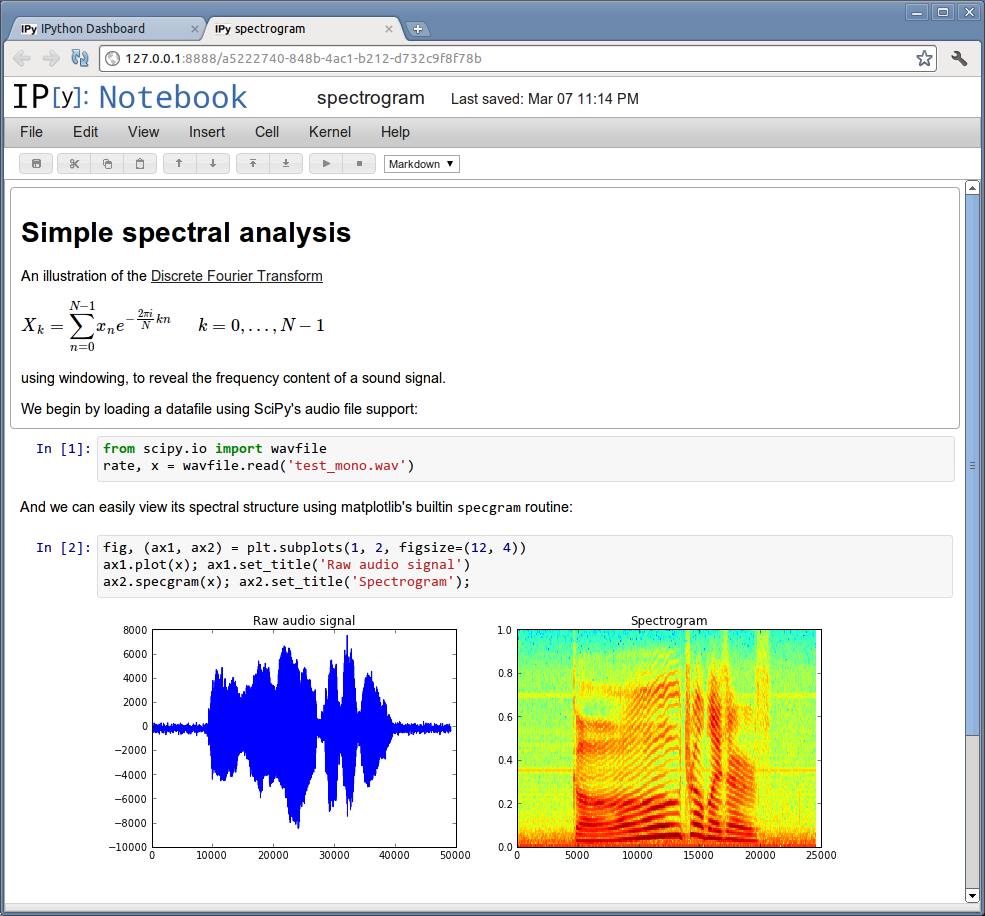
\includegraphics[width=3.2in]{fig/ipython-notebook-specgram.png}\par
  \end{centering}

  \caption{\label{fig:IPython-notebook}The web-based IPython Notebook combines
    explanatory text, mathematics, multimedia, code and the results from
    executing the code.}
\end{figure}

The driving idea behind the IPython Notebook is to enable researchers to move
fluidly between all the phases of the research life cycle we described earlier.
If the environment where they conduct their exploratory research can also
support all subsequent stages of this cycle, and does so while smoothly
integrating with the version control and process practices we've previously
espoused, the likelihood that a final published result will be reproducible
increases significantly.  The Notebook system is designed around two central
ideas: (a) an openly specified protocol to control an interactive computational
engine, and (b) an equally open format to record these interactions between the
user and the computational engine, including the results produced by the
computations.

Before diving into the specifics of these two ideas, we note that the above
design is independent of the Python language: while IPython started its life as
a Python-specific project, the vision of the Notebook system is
language-agnostic.  First, while working in Python, users can mark entire code
blocks for execution via a separate language by using a special syntax on the
block's first line: a user can for example start a block \texttt{\%\%R},
\texttt{\%\%octave}, \texttt{\%\%bash} or \texttt{\%\%ruby} and IPython will
execute the entire block with the respective system.  The development community
is also busy implementing similar support for even new and experimental
scientific languages such as Julia, enabling a user to control from a single
IPython notebook a workflow that combines most commonly used high-level
languages in modern scientific computing.  Second, an \emph{entire notebook}
can be executed in a different language if a remote engine (referred to as a
\emph{kernel}) exists that implements the interaction protocol.  As of this
writing, prototype kernels are being developed for Ruby, JavaScript, R and
Julia.

The IPython architecture provides a way to capture, version control, re-execute
and convert into other output formats, any computational session.  Notebooks
can be shared with colleagues in their native form for re-execution or
converted into HTML, \LaTeX, or PDF formats for reading and dissemination.  They
can be used in slideshow mode to give presentations that remain connected to a
live computation and can be exported into plain scripts for traditional
execution outside of the IPython framework.

The IPython protocol consists of messages in JSON (JavaScript Object Notation)
format that encode all actions that an interactive user can request of a
computational kernel, such as executing code, transferring data or sending
results, among many others.  While this protocol is implemented in IPython,
third-parties can independently implement it and provide new kernels that will
be able to interact with the notebook interface and clients.  The notebook file
format is a simple JSON data structure that contains a series of one or more
``worksheets'', each of which is a list of cells.  A cell can contain either
text or code, and code cells can also have the output corresponding to the
execution.  All sub-structures in the notebook format (the entire notebook, the
worksheets, and the individual cells) have attached flexible metadata
containers; this metadata can be used by post-processing tools.  The file
format stores the communication protocol's payloads unmodified, so it can be
thought of as a structured and filtered log (since the user chooses what to
keep while working interactively) of the computation.  

The IPython project has taken elements pioneered by the Mathematica and Sage
notebooks and created a generic protocol and file format to control and record
literate computing sessions in any programming language.  This was a deliberate
choice in contrast to the literate programming approach: by providing a tool
that operates close to the live workflow of research computing (in contrast to
the batch-processing mode encouraged by classic literate programming tools),
the resulting documents are immediately reproducible sessions that can be
published in their own right or as companion materials to a more traditional
manuscript.  Given how IPython also includes support for parallel computing,
which we don't discuss here in the interest of conciseness, the system provides
an end-to-end environment for the creation of reproducible research.

The real-world possibilities this offers were demonstrated during a
collaboration in 2012 between the IPython team, a microbiology team led by Rob
Knight from the University of Colorado and Greg Caporaso from the University of
Northern Arizona, and Justin Riley from MIT who created the StarCluster system
\footnote{\url{http://star.mit.edu/cluster/}} for deployment and control of
parallel resources on Amazon's EC2 cloud platform.  As part of an NIH-funded
workshop to explore the future of genomics data analysis in the cloud, this
combined team collaborated on creating a fully parallelized analysis comparing
the predictive behavior of different sizes and locations of gene sequence reads
when reconstructing phylogenetic trees.  The microbiologists had developed a
serial prototype of this idea using their Qiime libraries
\cite{caporaso2010qiime}, but a large-scale analysis with a full dataset would
require roughly a month of CPU time on a single workstation.  By locating the
IPython Notebook server on Amazon cloud instances, the entire team was able to
log into a single instance and by editing the code directly in the cloud, in a
single day turn this prototype into a set of production notebooks that would
execute the analysis in parallel using multiple Amazon servers.  Once the
parallel was tested, it became evident that there was not only an interesting
example of using cloud technologies for rapid development of research ideas but
also a biologically relevant finding; within a week the team had completed a
more extensive run using 24 hours of execution on 32 nodes and submitted a
manuscript for publication \cite{RWM+12}.  This paper is now accompanied by all
of the IPython notebooks that enable any reader to fully reproduce our
analysis, change parameters and question our assumptions, without having to
re-implement absolutely anything or be hampered by lack of access to the code
and data.  We have made available not only the final notebooks, but also the
Amazon Virtual Machine Images (data files that represent a virtual computer on
Amazon's cloud platform), so that the entire analysis can literally be
re-executed under identical conditions by anyone with an Amazon account.

This example, anecdotal as it may be, indicates there is validity in the vision
we propose here: that by providing tools that encompass the entire cycle of
research, from exploration to large-scale parallel production and publication,
we can provide the scientific community with results that are immediately
accessible to others and reproducible, seeding the continued evolution of the
research process.

The IPython project also has developed tools that make it very easy to share
and disseminate content created as notebooks in a variety of forms.  The
Notebook Viewer hosted at \url{http://nbviewer.org} is a system that can render
\emph{any} publicly available IPython notebook as a web page.  This enables
users to share notebooks with others by simply putting them online and
pointing them to the rendered webpage, without the readers having to install
anything on their own systems.  And the same technology that powers the
notebook viewer service can also generate HTML files suitable for inclusion in
other websites, in particular, blogs.  Since a lot of rapid technical
communication is happening today on the Internet via blogs, this is an
important aspect of linking reproducible research to the rapid feedback cycle
of web-based discussion.  With a single command, a user can convert a notebook
file into HTML ready for posting to a blog, and this is already being used by
scientists to write both short technical posts and also more complex
materials: Jose Unpingco, a researcher with the US Department of Defense, is
currently working on a book titled \emph{Python for Signal Processing}, and
this book is available during writing as a GitHub
repository\footnote{\url{https://github.com/unpingco/Python-for-Signal-Processing}}.
This repository contains a series of IPython notebooks so that readers can
directly execute the code in the book, and they are also being published as a
series of blog posts as they become available, at
\url{http://python-for-signal-processing.blogspot.com}, so readers can comment
and discuss with the author throughout the process of book development, but
they can do so based directly on the actual code that creates all the examples
in the book.

The signal processing book is, to our knowledge, the first example of a full
book being written as a collection of executable IPython notebooks, but this
follows a tradition created by Mathematica, whose documentation is itself a
collection of executable Notebooks.  Furthermore, in recent years Rob Beezer,
from the University of Puget Sound, has developed popular Introductory Linear
Algebra book \cite{beezer2009first} that is based on the Sage system and
also combines the mathematics and text with code that can be directly executed
and modified by the readers.  It seems clear to us that this ability to ``close
the loop'' between what the authors had on their screens and what their readers
can execute themselves is an important element of the movement towards
reproducibility in research.

As a concrete implementation of the ideas of reproducible research using the
tools we've described in this chapter, during the ongoing process of research
itself, we can point to work being carried by a collaboration where one of us
(FP) is a member, on novel ways to model the mathematical structure of the
signal generated by MRI devices in the imaging of water diffusion in the
brain.  This work, as yet unpublished, is being developed as an open repository
on GitHub\footnote{\url{https://github.com/fperez/spheredwi}} where all code
for our research is posted during writing, all computational experiments are
created as IPython notebooks, and submitted manuscripts are created directly
from the code and notebooks (along with additional narrative written by hand).
This is an experiment we are conducting precisely with the intent of showing
that it is viable to conduct research in an open and reproducible way, with all
history of the code and manuscripts being held in publicly visible repositories
that anyone can download and replicate even prior to publication. 

We close this section by noting that the above tools are also playing an
central role in the last stage of the cycle we outlined earlier, education.  We
will increase our chance that the next generation of scientists adopts improved
reproducibility practices if we educate them with the same tools that we use
for everyday research, and a couple of modern efforts that aim to bring
improved computational literacy to scientific research have adopted the IPython
notebook.  Software Carpentry\footnote{\url{http://software-carpentry.org}} is
a project funded by the Alfred P. Sloan Foundation and led by Greg Wilson at
the Mozilla Foundation whose motto is Richard Feynman's famous ``What I cannot
create, I do not understand.''  They produce, with rigorous follow-up and
assessment, workshops aimed at working scientists (typically graduate students
and postdoctoral researchers, but always open to broad audiences) and whose
purpose is to instill in them a collection of skills and best practices for
effectively using computing as a daily research tool.  The Software Carpentry
workshops cover topics ranging from the basics of the Unix shell to version
control, Makefile automation of processes and basics of scientific Python
including data analysis and visualization.  They have recently adopted the
IPython Notebook as the base system for teaching the scientific Python parts of
their curricula, and provide the IPython team with direct feedback on its
strengths and weaknesses as an educational tool.  In a similar vein, Josh Bloom
from the astronomy department at UC Berkeley has led, for a number of years, a
3-day workshops on the use of Python as a tool for scientific
computing\footnote{\url{http://pythonbootcamp.info}}.  These are open to the
entire campus community and followed by an optional for-credit seminar where
students learn more advanced skills for using Python as a research tool.  F.
Pérez and other members of the IPython team at UC Berkeley regularly lecture in
the bootcamp and courses, where the notebook is the means for delivery of
course materials and interactive lecturing.  While we have identified a number
of weaknesses and areas for improvement, we have also found this environment to
be markedly superior to all previous tools we had used in the past for teaching
in similar contexts.

As these capabilities in IPython reach wider usage, with scientists now
developing complete books and lecture series based on the system, we are
considering a number of new challenges and questions introduced by these
capabilities.  The interactive computing model is a fluid and natural one, but
we need to find ways to extend it into the development of longer-term
production codes that are robust, documented, tested and integrated into
reusable libraries.  This means bridging the gap between a 'scripting'
mentality and a 'developer' one, and while we have already made progress on
that front in IPython, many questions remain open for the future.  This is an
example of how we need to start thinking about software with the same care as
the scientific process it supports.

In summary, IPython embodies the main ideas we've woven into our discussion: it
was born out of the interplay between everyday scientific research and open
source software development, and it tries to be a natural part of the entire
research cycle in order to make it more fluid, efficient, and reproducible.

\section{Conclusion}\label{conclusion}

As research grows increasingly dependent on computing, it becomes critical for
our computational resources to be developed with the same rigor, review,
and access as the results they support. In particular, we believe that
reproducibility in computational research requires: (1) sharing of scientific
software, data, and knowledge necessary for reproducible research; (2)
readable, tested, validated, and documented software as the basis for reliable
scientific outcomes; (3) high standards of computational literacy in the
education of mathematicians, scientists, and engineers; and (4) open source
software developed by collaborative, meritocratic communities of practice.

Achieving these goals won't be easy.  It requires changing the educational
process for new scientists, the incentive models for promotions and rewards,
the publication system, and more. In this chapter, we focused on the need for
an open source ecosystem for scientific computing developed by communities of
practice. \fix{finish summarizing and hint at next steps}


%\begin{itemize}
%\item Levels of reproducibility: replication, validation, reproduction,
%new construction.
%\item Conditions: clarity, transparency and trace-ability, predictability
%(which requires automation), communicability
%\end{itemize}
%
%While the mechanical reproduction of computational results is not a
%panacea in itself; the rigor, openness, culture of validation, collaboration and
%other aspects of science must become a routine part of our computational practices.


%This is a large and complex problem that requires changing the educational
%process for new scientists, the incentive models for promotions and
%rewards, the publication system, and more.

\section*{Acknowledgments}

\fix{please review this and make sure we have thanked everyone}

We would like to thank all the members of the scientific Python community as
well as the many scientist from various labs whose work and ideas have inspired
the ideas we've presented here.  John D. Hunter, to whom this chapter is
dedicated, created the matplotlib graphics library that has been a central
pillar of the Scientific Python ecosystem; his tragic early passing in 2012 was
a personal blow to the authors as well as a loss to our community.  Brian
Granger and Min Ragan-Kelley have worked closely with F.P. on the development
of IPython for a number of years and are responsible for many of the ideas that
the project embodies.  Matthew Brett is a colleague who \fix{what else about
  matthew?}.  Titus Brown, Vincent Carey, Paul Ivanov, Jean-Baptiste Poline,
and Stéfan van der Walt provided valuable feedback on drafts of this chapter.


\bibliographystyle{plain}
\bibliography{repro-chapter}

\end{document}
